In order to test how well our mapping can keep the relation between objects, we made a small setup on a table.

\begin{figure}[H]
	\centering
	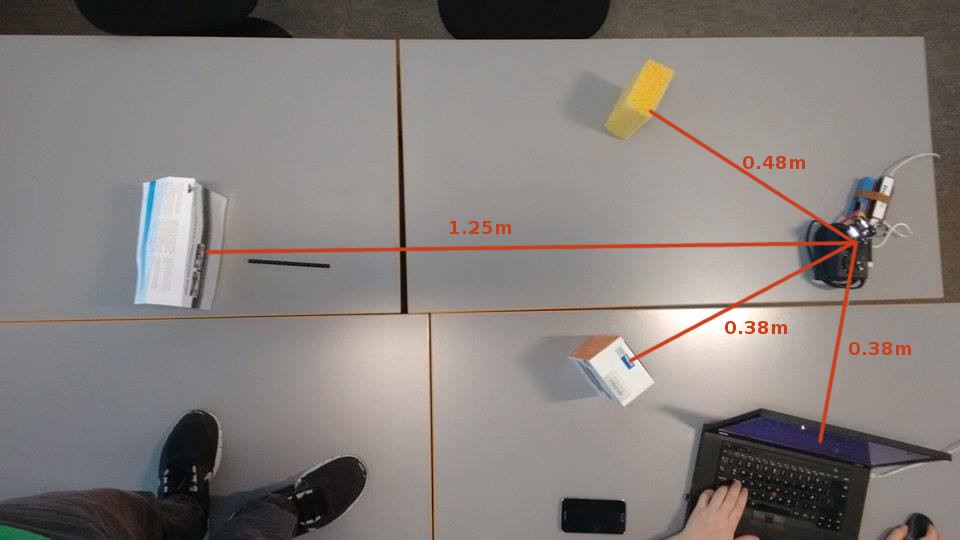
\includegraphics[scale=.4]{images/h101-photo.jpg}
	\caption{A photo of room H101 that was mapped.}
	\label{fig:internallidar}
\end{figure}

This figure shows what the setup was, with the addition of some distances.


\begin{figure}[H]
	\centering
	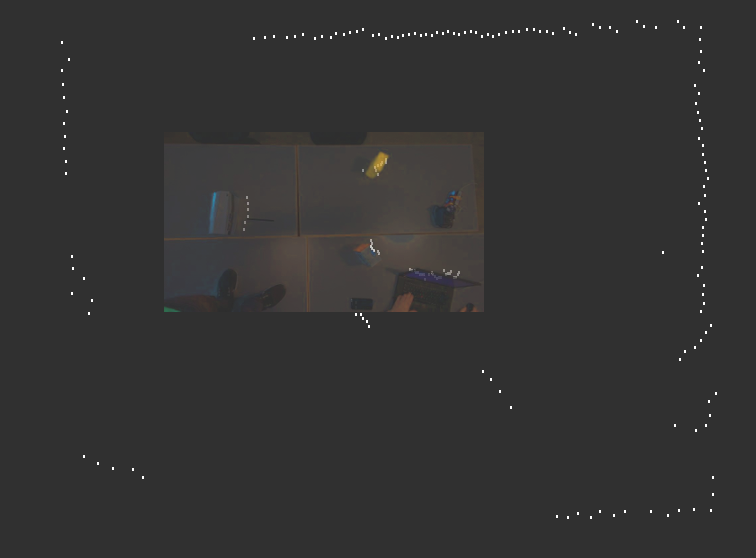
\includegraphics[scale=.4]{images/h101_obstacles_overlay.png}
	\caption{A map of room H101 with some small obstacles.}
	\label{fig:internallidar}
\end{figure}

This is the map that was generated by the laser, roughly overlayed with the picture of the setup.

Just from this very rough overlayed picture, it is easy to see that our map keeps the aspect-ratio of the physical world that it is mapping. 
